\documentclass[11pt]{article}
	
	\usepackage{adjustbox}
	\usepackage{amsmath}
	\usepackage{amssymb}
	\usepackage{float}
	\usepackage[T1]{fontenc}
	\usepackage{graphicx}
	\usepackage{hhline}
	\usepackage[utf8]{inputenc}
	\usepackage{mathtools}
	\usepackage{multicol}
	\usepackage{multirow}
	\usepackage{wasysym}
	\usepackage[paperheight=27.94cm,paperwidth=21.59cm,left=2.54cm,right=2.54cm,top=2.54cm,bottom=2.54cm]{geometry}
	
	
	\setlength\parindent{0pt}
	\renewcommand{\arraystretch}{1.3}
	
	
	\title{Proces adiabatic}
	
	\begin{document}
	\maketitle
	
	\begin{center}
	Paliciuc Cosmin-Constantin 313AC
	\end{center}
	
	
	{\footnotesize Un proces adiabatic sau transformare adiabaticăeste o transformare a unui sistem termodinamic în care nu se produce un schimb de căldură cu exteriorul.\par}
	
	\section{Proces adiabatic}
	
	Primul principiu al termodinamicii afirmă că energia este conservată. Pentru un sistem fizic macroscopic în repaus (variația energiei cinetice este zero), variația energiei interne a sistemului este egală cu energia schimbată cu mediul extern. Acest schimb se poate face într-un mod ordonat prin lucrarea de forțe ( de transfer de energie mecanică) sau dezordonate prin transfer termic de căldură (transfer de energie termică agitare). Pentru o transformare elementară (adică care dă naștere unei mici variații a parametrilor care descriu sistemul). Prin urmare, un proces adiabatic este o transformare fără transfer de căldură, adică . Variația energiei interne a sistemului este egală cu singurul transfer de energie mecanică prin activitatea forțelor aplicate sistemului.
	
	\section{Ecuația transformării adiabatice}
	
	Transformarea adiabatică a gazului ideal poate fi descrisă de ecuația (1) unde p este presiunea, V este volumul, iar (doar pentru gaze perfecte):\( \gamma  =\frac{C_{p}}{C_{v}} =\frac{i+2}{i}\)
	
	\( C_{p}\) fiind capacitatea termică masică la presiune constantă, \( C_{V}\)  fiind capacitatea termică masică la volum constant, \( \gamma\) este exponentul adiabatic, iar \textit{i} reprezintă numărul gradelor de libertate ale gazului. \textit{i} poate fi 3 pentru gazele monoatomice, 5 pentru cele biatomice și 6 pentru celelalte gaze.
	
	\begin{equation}
	pV^{\gamma } = constant
	\end{equation}
	
	
	\vspace{1\baselineskip}
	\textbf{Tabelul 1. }Variația presiunii în funcție de volum
	
	\begin{table}[H]
	\begin{adjustbox}{max width=\textwidth}
	\begin{tabular}{p{1.99cm}p{7.0cm}p{7.5cm}}
	\hline
	\multicolumn{1}{|p{1.99cm}}{\textit{Nr.crt}} & 
	\multicolumn{1}{|p{7.0cm}}{\textit{Mărime}} & 
	\multicolumn{1}{|p{7.5cm}|}{\textit{Valoare}} \\ 
	\hline
	\multicolumn{1}{|p{1.99cm}}{1} & 
	\multicolumn{1}{|p{7.0cm}}{presiune} & 
	\multicolumn{1}{|p{7.5cm}|}{1 atm} \\ 
	\hline
	\multicolumn{1}{|p{1.99cm}}{2} & 
	\multicolumn{1}{|p{7.0cm}}{volum} & 
	\multicolumn{1}{|p{7.5cm}|}{200 l} \\ 
	\hline
	\end{tabular}
	\end{adjustbox}
	\end{table}
	\begin{table}[H]
	\begin{adjustbox}{max width=\textwidth}
	\begin{tabular}{p{16.49cm}}
	\hhline{~}
	\multicolumn{1}{p{16.49cm}}{\centering\ \ \ \ 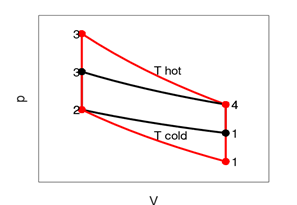
\includegraphics[width=7.85cm,height=5.42cm]{Picture1.png}
	\ \ \ \ \ \ \ \ } \\ 
	\hhline{~}
	\multicolumn{1}{p{16.49cm}}{\centering
	\textbf{Figura 1.} Curba ce reprezintă variația presiunii în funcție de volum} \\ 
	\hhline{~}
	\end{tabular}
	\end{adjustbox}
	\end{table}
	\vspace{1\baselineskip}
	Curba ce reprezintă variația presiunii în funcție de volum pentru transformarea adiabatică se numește adiabată.
	
	\section{Concluzii}
	
	Transformarea adiabatică este un proces termodinamic în care sistemul termodinamic se schimbă dintr-o stare inițială într-o altă stare finală, fără a exista transfer de căldură între sistem și mediul extern. Acest lucru înseamnă că sistemul termodinamic nu primește nicio cantitate de căldură de la mediul extern și nici nu cedează căldură către mediul extern.
	
	
	\textbf{Bibliografie}
	
	1 Bazil Popa (coord.), Manualul inginerului termotehnician, vol. 1, București: Editura Tehnică, 1986
	
	2 Ioan Vlădea, Tratat de termodinamică tehnică și transmiterea căldurii, București: Editura Didactică și Pedagogică, 1974
	\end{document}